\documentclass{article}
\usepackage[UTF8]{ctex}
\usepackage[T1]{fontenc}
\usepackage[utf8]{inputenc}
\usepackage{titlesec}
\usepackage[colorlinks, linkcolor = black]{hyperref}
\usepackage{float}
\usepackage{xcolor}
\usepackage{amsmath}
\usepackage{amssymb}
\usepackage{latexsym}
\usepackage{amsthm}
\usepackage{graphicx}
\usepackage{enumerate}
\usepackage{enumitem}
\usepackage{tikz}
\usepackage{subcaption}
\usetikzlibrary{positioning}
\usetikzlibrary[arrows, shapes, chains]
\renewcommand*\thesubfigure{\roman{subfigure}}
\setlist{
    leftmargin = .1\linewidth,
    % rightmargin = .1\linewidth,
    % label=\emph{\alph*}.
}

\titleformat{\section}[block]{\LARGE\scshape}{\arabic{section}}{1em}{}[]

\title{Homework 7}
\author{PB17000297 罗晏宸}
\date{April 19 2020}

\begin{document}
\maketitle

\section{Exercise 14.12}
两个来自世界上不同地方的宇航员同时用他们自己的望远镜观测了太空中某个小区域内恒星的数目$N$。他们的测量结果分别为$M_1$和$M_2$。通常,测量中会有不超过 1 颗恒星的误差,发生错误的概率$e$很小。每台望远镜可能出现(出现的概率$f$更小一些)对焦不准确的情况(分别记作$F_1$和$F_2$),在这种情况下科学家会少数三颗甚至更多的恒星(或者说,当$N$小于 3 时,连一颗恒星都观测不到)。考虑图\ref{14.22}所示的三种贝叶斯网络结构。
\begin{figure}
    \centering
    \begin{subfigure}[t]{0.3\textwidth}
        \centering
        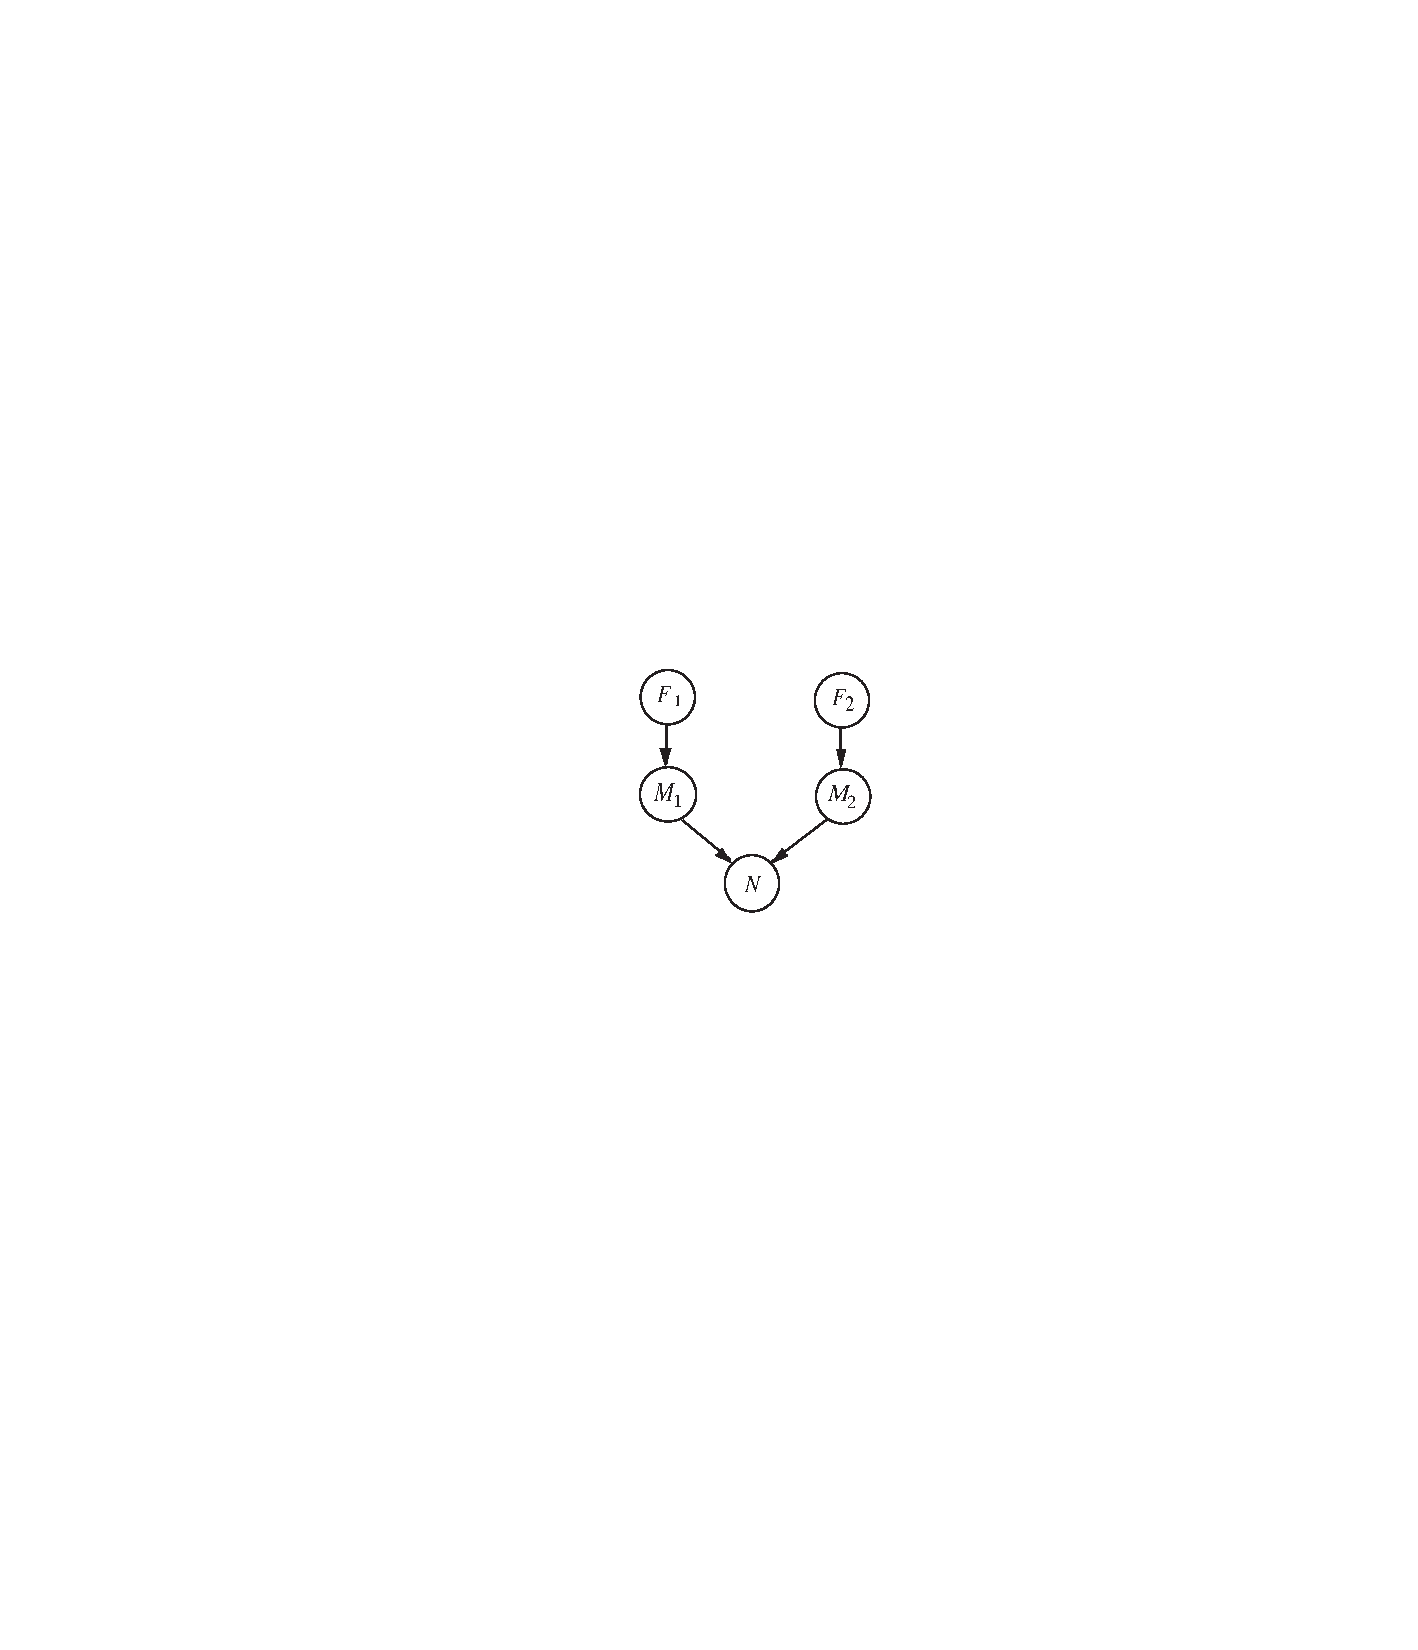
\includegraphics[scale = 0.6]{Figure/14-22(i).pdf}
        \caption{}
        \label{14.22(i)}
    \end{subfigure}
    \begin{subfigure}[t]{0.3\textwidth}
        \centering
        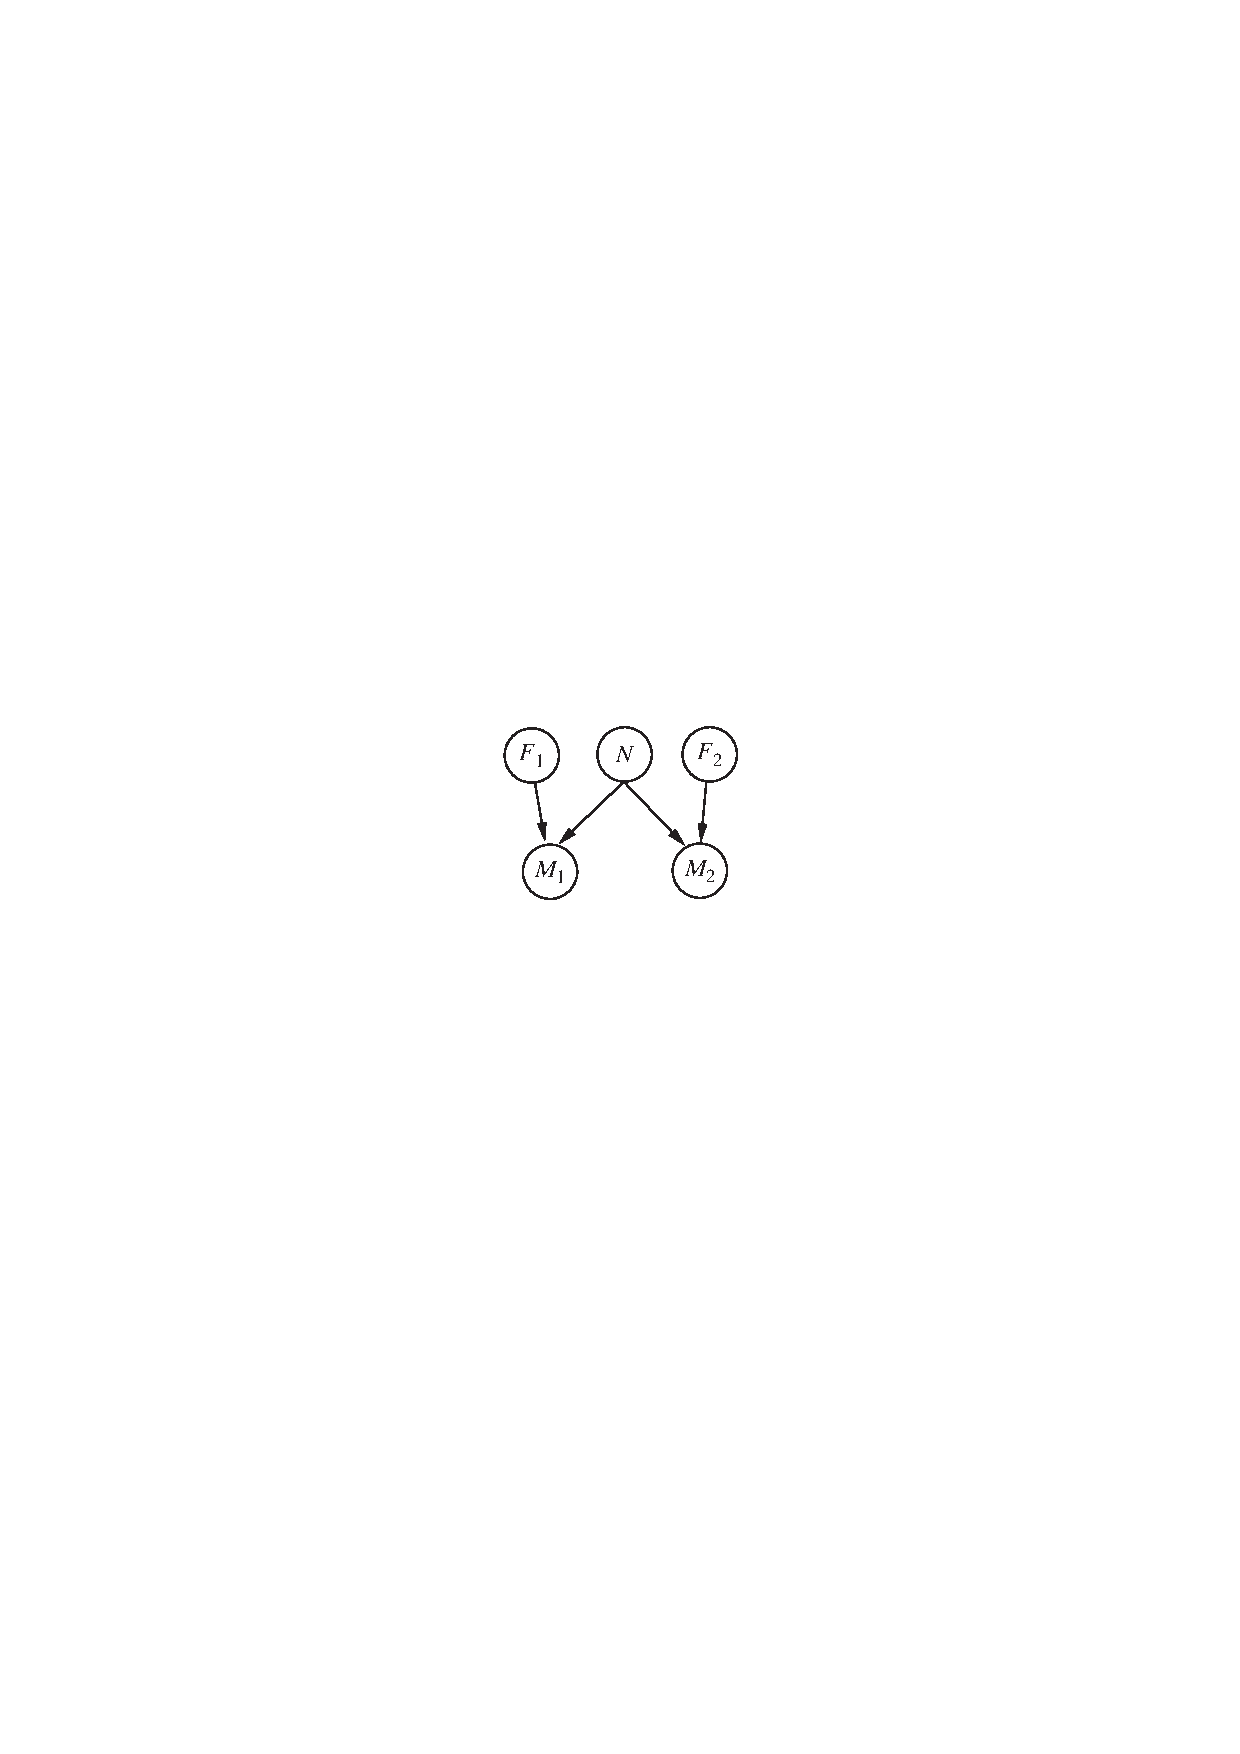
\includegraphics[scale = 0.6]{Figure/14-22(ii).pdf}
        \caption{}
        \label{14.22(ii)}
    \end{subfigure}
    \begin{subfigure}[t]{0.3\textwidth}
        \centering
        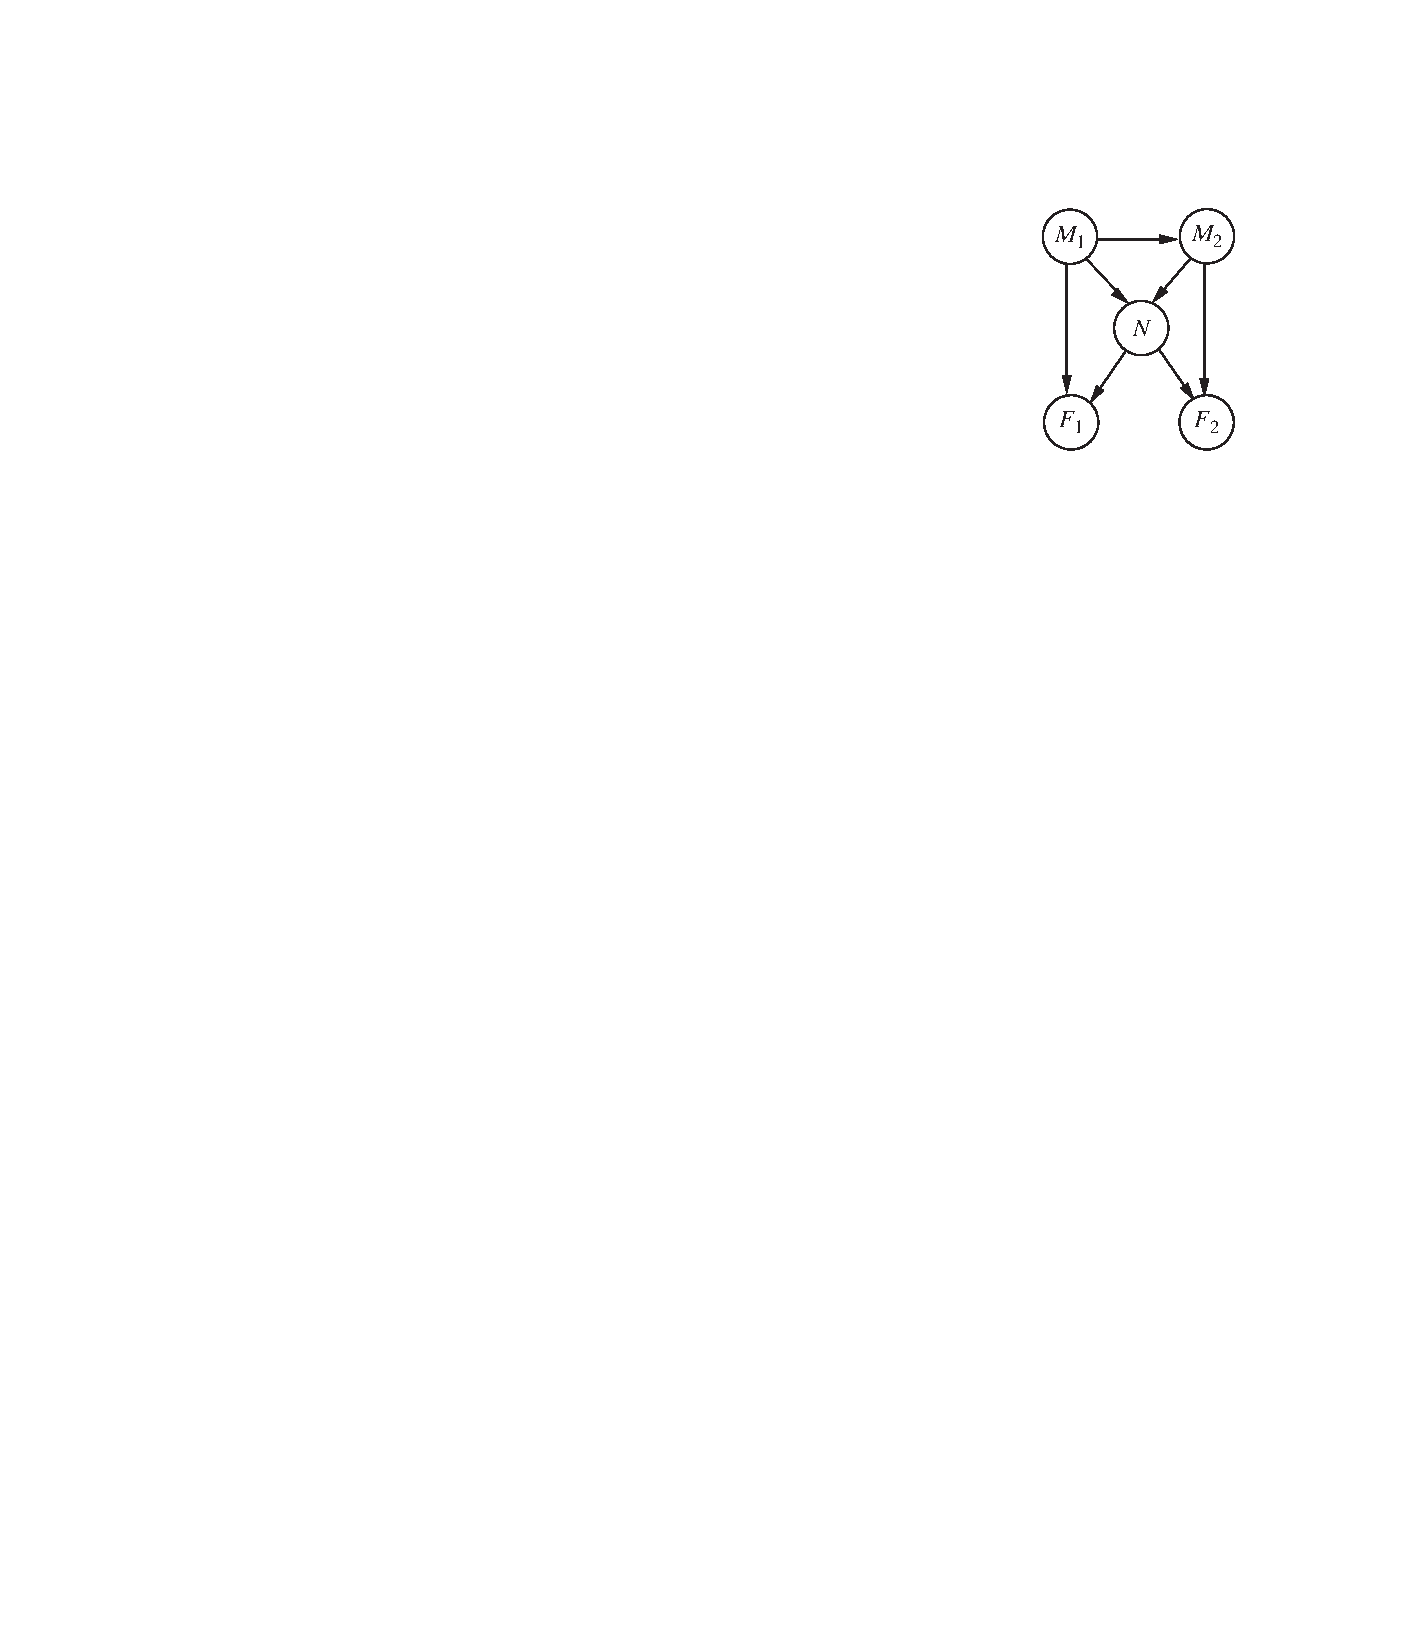
\includegraphics[scale = 0.6]{Figure/14-22(iii).pdf}
        \caption{}
        \label{14.22(iii)}
    \end{subfigure}
    \caption{望远镜问题的三种可能网络}
    \label{14.22}
\end{figure}
\subparagraph{a.} 这三种网络结构哪些是对上述信息的正确(但不一定高效)表示?
\subparagraph{b.} 哪一种网络结构是最好的?请解释。
\subparagraph{c.} 当$N \in \{1,\, 2,\, 3\}$,$M_1 \in \{0,\, 1,\, 2,\, 3,\, 4\}$时,请写出$\mathbf{P}(M_1 | N)$的条件概率表。概率分布表里的每个条目都应该表达为参数$e$和/或$f$的一个函数。

\paragraph{解}
\subparagraph{a.}
\subparagraph{b.}
\subparagraph{c.}

\section{Exercise 14.13}
考虑图\ref{14.22}(\subref{14.22(ii)})的网络,假设两个望远镜完全相同。$N \in \{1,\, 2,\, 3\}$,$M_1,\, M_2 \in \{0,\, 1,\, 2,\, 3,\, 4\}$,CPT 表和习题14.12所描述的一样。使用枚举算法(图\ref{14.9})计算概率分布$\mathbf{P}(N | M_1 = 2,\, M_2 = 2)$。
\begin{figure}
    \centering
    \fbox{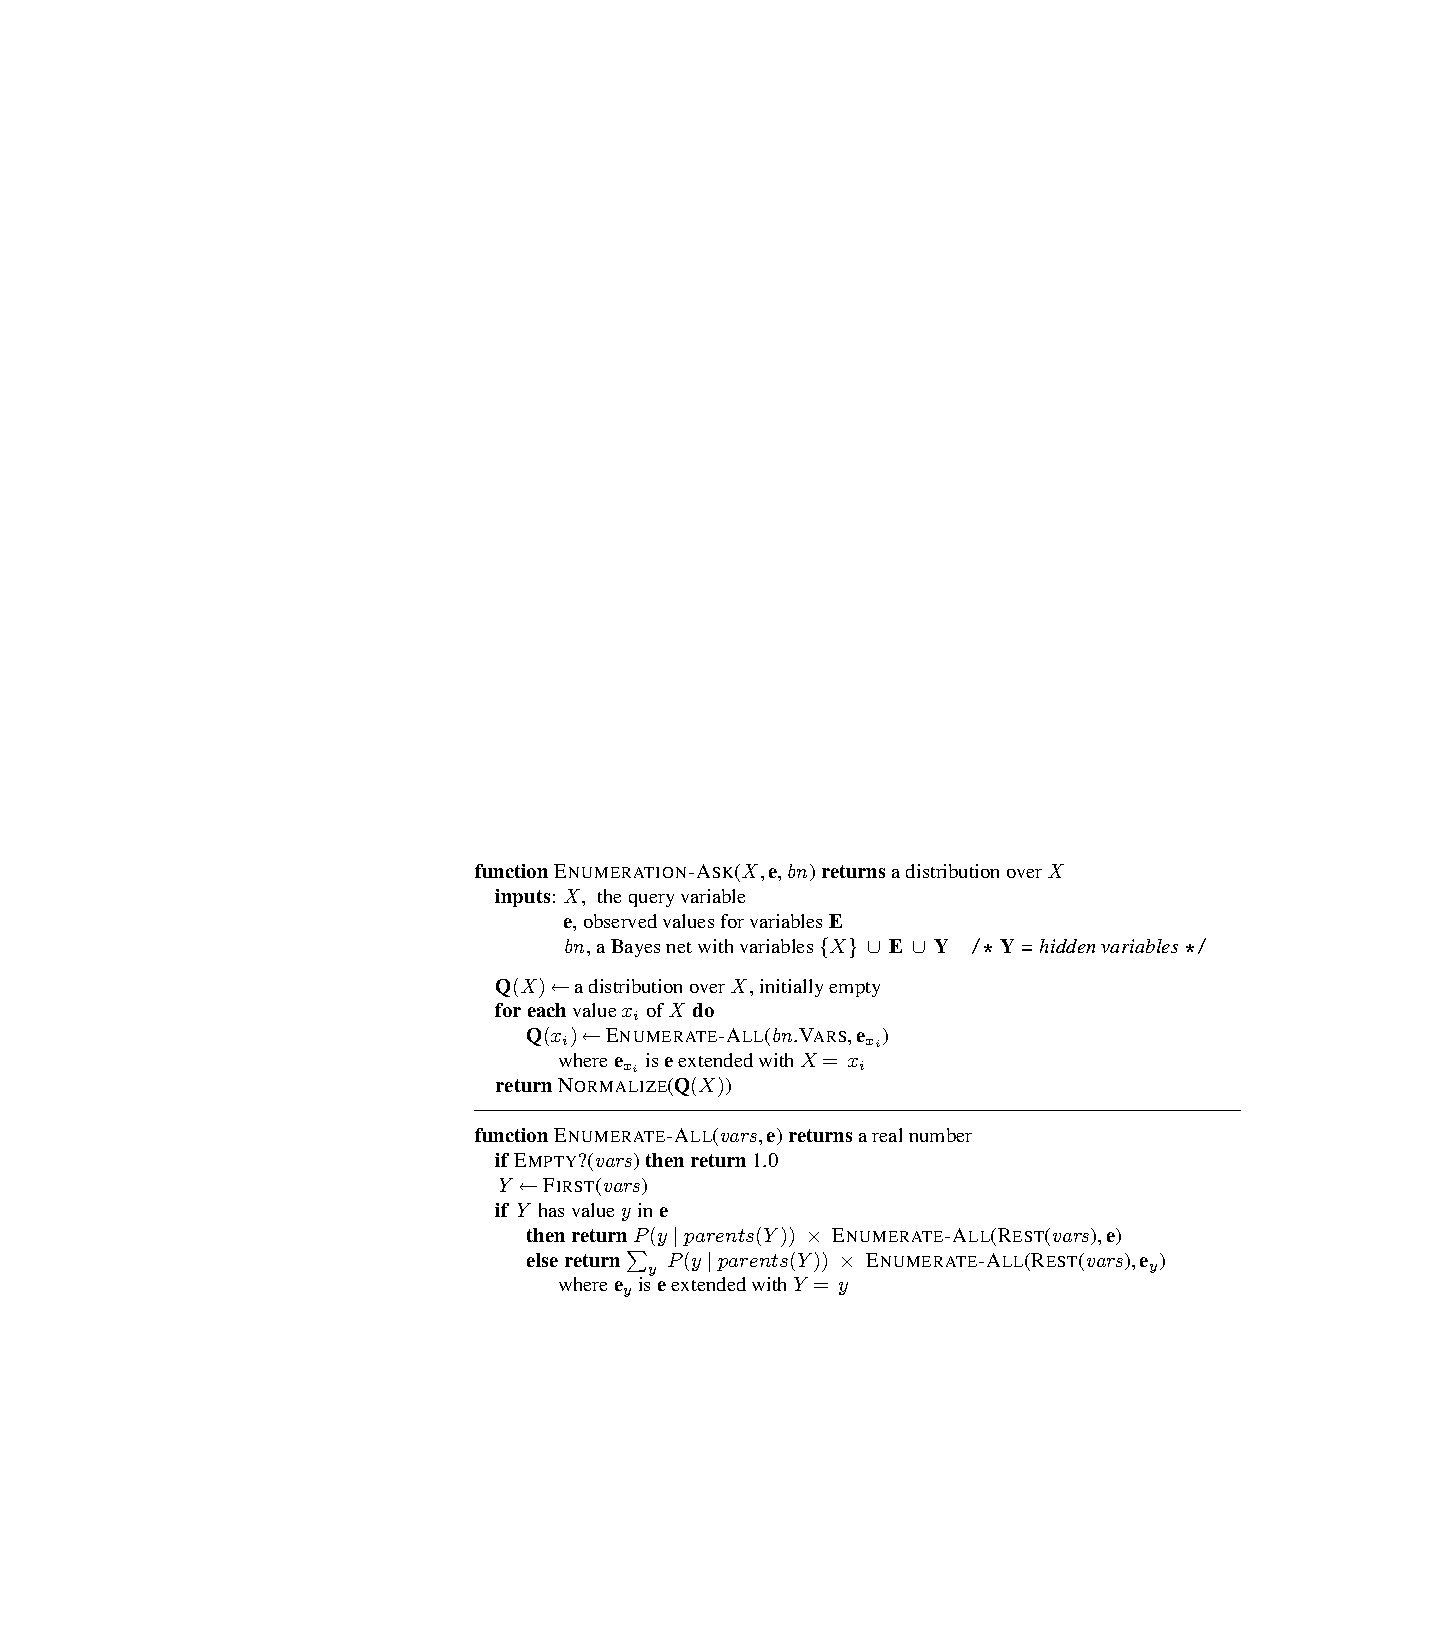
\includegraphics[scale = 0.83]{Figure/14-9.pdf}}
    \caption{在贝叶斯网络上回答查询的枚举算法}
    \label{14.9}
\end{figure}
\paragraph{解}

\section{Exercise 14.15}
考虑图\ref{14.11}中的变量消元算法。
\begin{figure}
    \centering
    \fbox{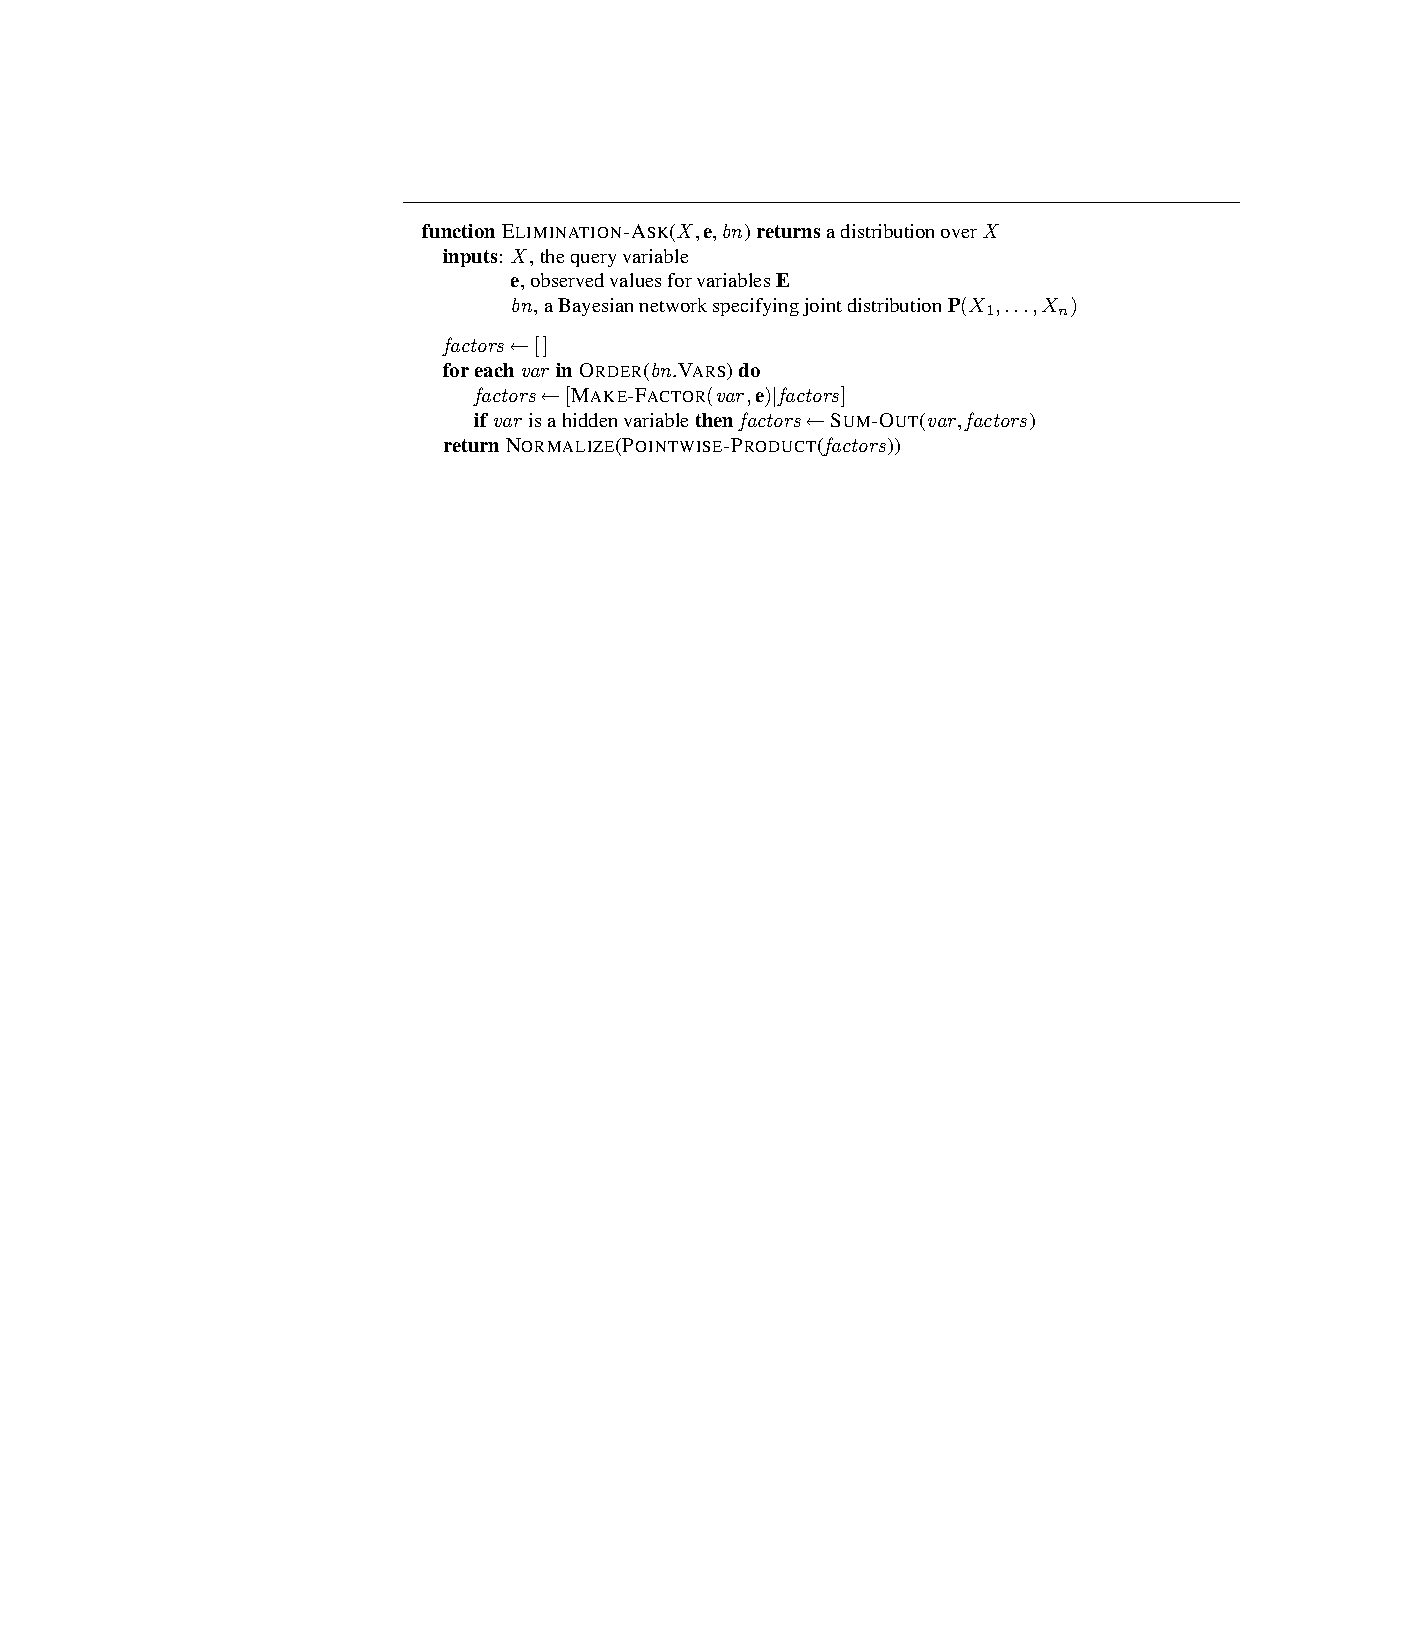
\includegraphics[scale = 0.83]{Figure/14-11.pdf}}
    \caption{用于贝叶斯网络推理的变量消元算法}
    \label{14.11}
\end{figure}
\subparagraph{a} 14.4节对如下查询应用了变量消元算法$$\mathbf{P}(\textit{Burglary} | \textit{JohnCalls} = \textit{true},\, \textit{MaryCalls} = \textit{true})$$执行必要的计算,并检验计算结果的正确性。
\subparagraph{b} 统计所执行的算术运算的次数,将其与枚举算法所需的运算次数进行比较。
\subparagraph{c} 假设贝叶斯网络结构具有链式结构,即由一个布尔随机变量序列$X_1,\, \cdots,\, X_n$构成,其中$\textit{Parents}(X_i) = \{X_{i - 1}\},\ i = 2,\, \cdots,\, n$。请问使用枚举算法计算$\mathbf{P}(X_1 | X_n = \textit{true})$的复杂度是多少?使用变量消元算法呢?

\paragraph{解}
\subparagraph{a}
\subparagraph{b}
\subparagraph{c}

\end{document}